\chapter{Supporting Multiple Users}

This chapter describes a new version of the Gabriel software framework that we
developed for WCA applications.
Next, it examines DNNs that can be run on mobile devices, and the tradeoffs of
using these models for WCA applications (in place of more accurate models that
can only be run on cloudlets).
Shifting computation from cloudlets to mobile devices reduces the bandwidth and
latency consumed by each WCA application user.

\section{Software Framework}

We developed a set of software libraries for WCA applications, called
Gabriel~\cite{gabriel_github}.
The primary feature of these libraries is to transmit data from mobile devices
to cloudlets.
WCA applications require responses shortly after a user completes a step, so
we always want to process the newest frame possible. We never want to build up
a queue of stale data to process. The library accomplishes this using a flow
control mechanism similar to the one proposed by \citet{ha2014}.

\subsection{Motivation}

The library we developed replaces an earlier implementation.
The code for this earlier implementation had become unmanageable.
It was tightly coupled around sending single image frames, and we
wanted the ability to send chunks of consecutive frames.
We also needed multiple clients to share one cloudlet, which the old code did
not support.
Developing a new version of the platform allowed us to use modern technologies
such as Python 3, WebSockets, and asyncio.
A key goal with the new version of the platform was making it easy to work with.
We published server and client libraries to package repositories, so that
developers can easily include them in Python and Android code.
Our code includes a special case for Gabriel workflows that involve a single
cognitive engine, which allows this engine to be run with the server in the same
Python program.

\subsection{Implementation Details}

We use the abstractions of ``sources'' and ``cognitive engines.'' A source is
anything that produces data on a mobile device. It could be a stream from a
sensor such as a camera or microphone. A source might also be a filter that runs
on the device, analyzes all frames produced by a sensor, but then only forwards
some of these frames to the
cloudlet. We use the term ``early discard'' to refer to filters like
this. A cognitive engine runs on a cloudlet and processes data. A cognitive
engine will process one frame of data at a time. A frame could be a single
image, a short clip of audio and/or video, or set of readings from a different
type of sensor.

All of the wearable cognitive assistance applications we have developed just
have a single cognitive engine processing images from a single camera source.
However, our framework supports workloads with multiple sources and multiple
cognitive engines. Multiple cognitive engines may consume data from the same
source, but we restrict each cognitive engine to consuming data from one source.
This reduces the complexity of cognitive engines.

Cognitive engines are all implemented in Python. Developers implement a single
function that takes a frame as its input parameter and returns a list of
results when it completes. Cognitive engines that do not need to return results
to mobile devices can just return an empty list.

\subsubsection{Flow Control}

Our flow control mechanism is
based on tokens. Clients have a set of tokens for every source. When a client
sends a frame to the cloudlet, it gives up a token for this source. The cloudlet
returns the relevant token when the function processing the frame returns.
A client will drop all frames from a source, until it gets a token for this
source. Clients and
cloudlets communicate using the The WebSocket Protocol~\cite{websocket}, which
is built on TCP.
Therefore, tokens will never be lost due to packet loss.

Applications that are very latency sensitive, such as
wearable cognitive assistance, will be run with a single token per source.
Applications that can tolerate higher latency can be run with more tokens.
Multiple tokens
will allow frames to be transmitted while the cloudlet is busy processing other
frames. This may cause frames to be buffered on the cloudlet, if the
cognitive engine takes a long time to process earlier frames. As a result, there
might be a significant amount of time between when a frame is captured and when
it gets processed. However, using multiple tokens does avoid periods where the
cloudlet does not have any frames to process because it is waiting for the next
frame to be sent over the network. Increasing
the number of tokens thus increases the possible delay before a frame gets
processed but reduces the amount of time the cloudlet has no frames to process,
when network latency is high.
The number of tokens is thus a parameter that will
increase the framerate for applications that can tolerate higher latency.

When multiple cognitive engines consume frames from the same source, the token
for a frame is returned when the first cognitive engine finishes processing the
frame. A Client will only receive a result from the first cognitive engine that
finishes processing a frame, and it will not get additional results or tokens
when other engines finish processing the same frame. Our server library keeps a
queue of input frames for each source. When multiple clients produce frames from
the same source, such as two smartphones both capturing images with a camera,
these frames are put into the same queue. A cognitive engine will process the
frame at the head of the queue for the source it consumes frames from. This
frame will be left at the head of the queue, so other cognitive engines that
consume frames from the same source will also process it. This frame is only
removed from the queue when a cognitive engine finishes processing it. The
engine that finishes processing the frame at the head of the queue will be the
first to get the next frame in the queue (if there is one).

This mechanism ensures that frames get consumed at the
rate that the fastest cognitive engine can process them. If every cognitive
engine took a frame from the queue without leaving it for other engines, a
slower engine would process frames that the fastest engine does not.
This method also ensures that cognitive engines do not get stale
frames because they are slow. Cognitive engines always process the frame at the
head of the queue. If one engine is slow, and the queue gets advanced several
times while the slow engine is processing a single frame, the slow engine
ignores the frames it missed. Once this engine becomes free, it will start
processing the frame at the head of the queue at that time.

\subsubsection{Components}

Almost all of our applications use a single cognitive engine. Our server code
runs workflows like this as a single Python program. A WebSocket server is run
in the main process, and the cognitive engine is run in a separate process using
Python's multiprocessing module. Inter-process communication is done using the
multiprocessing module's Pipe function. For workloads that require multiple
cognitive engines (such as the one depicted in
Figure~\ref{fig:runtime_architecture}),
the WebSocket server is run as a standalone Python program and each cognitive
engine is run as a different Python program. The Python programs communicate
with each other using ZeroMQ~\cite{zmq}.

\begin{figure}[h!]
  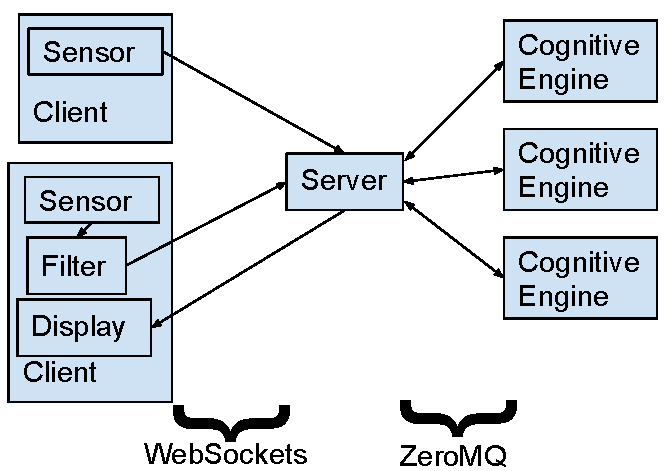
\includegraphics[width=8cm]{figures/runtime_architecture.pdf}
  \caption{A Gabriel workflow with two clients and three cognitive engines.
  }\label{fig:runtime_architecture}
\end{figure}

We have developed client libraries for Python and Android. These include
networking components that communicate with our server code using WebSockets.
The libraries also contain functions to capture images with a camera and
transmit the latest frame whenever a token is available. The Python library uses
OpenCV~\cite{opencv_library} to capture images while the Android library uses
CameraX~\cite{camerax}. Our Python code has been published to The Python Package
Index (PyPI)~\cite{gabriel_server, gabriel_python_client} and our Android code
has been published to Maven Central~\cite{gabriel_android_client}.

\section{Leveraging Mobile Device Hardware}

This section considers running some or all of the computations for WCA
applications on mobile devices instead of cloudlets.

\subsection{Accuracy Comparisons}

We compare the accuracy of models and model pairs that developers can use in WCA
applications.
Some of these models can be run directly on mobile devices or on cloudlets,
while others can only be run on cloudlets.

\subsubsection{Running a Single Model}\label{sec:single_model}

In an attempt to develop extremely lightweight versions of our applications,
we considered using a single DNN, rather than the pipeline described in
\S\label{sec:two_stage}.
We used data from four of our applications, which is summarized in Table~TODO.
The training set contains images that were labeled with a bounding box around
the subassembly.
The test set contains images that are distinct from the training set, but were
not labeled with bounding boxes.
All images in the training and test sets were assigned a class label, indicating
the step of the task that was shown in the image.

For each application, we trained a Resnet 50~\cite{He2016} image classifier,
three different sized EfficientDet~\cite{Tan2020} object detectors, a
Fast MPN-COV~\cite{Li_2018_CVPR} classifier, and a standalone Faster
R-CNN~\cite{frcnn} object detector.
The size of a DNN refers to the number of nodes in the network.
We then evaluated these models on the test set for the relevant application.
When evaluating object detection results, we ignored bounding box coordinates
and just checked if the class label for the detected object with the highest
confidence score was correct.
Table~\ref{tab:standalone_accuracy} lists the accuracy of these models.

\begin{table}
\begin{tabular}{|l||l|l|l|l|}
\hline
  & Meccano & Stirling & Sanitizer & Toyplane\\
  \hline
  \hline
  Resnet 50 & 69.8\% & 26.3\% & 68.3\% & 56.4\%\\
  EfficintDet-Lite0 & \textbf{75.2\%} & 53.65\% & 79.3\% & 51.1\%\\
  EfficintDet-Lite1 & 71.1\% & \textbf{53.8\%} & 84.1\% & 63.5\%\\
  EfficintDet-Lite2 & \textbf{75.2\%} & 49.6\% & 84.9\% & 59.8\%\\
  \hline
\end{tabular}
  \caption{
    Classification accuracy for standalone DNN models.
    Accuracy is the percentage of images that the model classified correctly.
    The highest accuracy for each application is in bold.
  }\label{tab:standalone_accuracy}
\end{table}

\subsubsection{Running a Pipeline of Models}

The results in Table~\ref{tab:standalone_accuracy} leave a lot of room for
improvement.
We next evaluated an object detector and an image classifier used in a pipeline,
as described in \S\ref{sec:two_stage}.
The image classifiers from \S\ref{sec:single_model} were trained and tested
on uncropped images, while the image classifiers in our pipeline setup were
trained on images that were cropped to just contain the subassembly.
When testing the pipeline, we ran the object detector on uncropped images.
Then, we cropped the image around the bounding box returned by the object
detector, and then ran the image classifier on this cropped image.
Figure TODO shows an examples of cropped and uncropped images.
The results of these pipelines are presented in
Table~\ref{tab:pipeline_accuracy}.

\begin{table}
\begin{tabular}{|l||l|l|l|l|}
  \hline
  & Meccano & Stirling & Sanitizer & Toyplane\\
  \hline
  \hline
  EfficientDet-Lite0 and Resnet 50 & 75.0\% & 85.1\% & 87.9\% & 69.8\%\\
  EfficientDet-Lite0 and Fast MPN-COV & 82.0\% & 78.4\% & 79.3\% & 77.2\%\\
  EfficientDet-Lite1 and Resnet 50 & 74.6\% & 70.3\% & 87.7\% & 70.9\%\\
  EfficientDet-Lite1 and Fast MPN-COV & 81.7\% & 66.6\% & 79.3\% & 77.7\%\\
  EfficientDet-Lite2 and Resnet 50 & 75.0\% & \textbf{91.0\%} & 89.1\% & 70.1\%\\
  EfficientDet-Lite2 and Fast MPN-COV & 81.5\% & 86.0\% & 80.6\% & 76.6\%\\
  Faster R-CNN and Fast MPN-COV & \textbf{84.5\%} & 80.9\% & \textbf{92.9\%} & \textbf{81.9\%}\\
  \hline
\end{tabular}
  \caption{
    Classification accuracy for pipelines consisting of an object detector,
    followed by an image classifier.
    Accuracy is the percentage of images that the model classified correctly.
    The highest accuracy for each application is in bold.
  }\label{tab:pipeline_accuracy}
\end{table}

The accuracy of the best pipeline was better than the accuracy of the best
standalone DNN for all of our applications.
Faster R-CNN and Fast MPN-COV was the best pipeline for all of our applications
except Stirling.

\subsection{WCA Without Cloudlets}

The EfficientDet~\cite{Tan2020} object detector and Resnet 50~\cite{He2016}
image classifier can be run on certain Android devices using TensorFlow Lite.
This allows developers to create WCA applications that run some or all of their
computations on mobile devices instead of cloudlets.
However, Fast MPN-COV and Faster R-CNN cannot currently run on mobile
devices~\cite{tflite, torchscript}.
We developed versions of our applications that ran EfficientDet and Resnet 50
pipelines directly on mobile devices.

We profiled our applications on the three devices listed in
Table~\ref{tab:devices}.
All three devices run Android, which allowed us to re-use our code for all three
tests.

\begin{table}
\begin{tabular}{|l||p{4cm}|p{3cm}|p{3.5cm}|}
  \hline
  Device & Google Glass Enterprise Edition 2 & Magic Leap 2 & Vuzix Blade 2\\
  \hline
  \hline
  Year Launched & 2019 & 2022 & 2022\\
  Weight & 46g (without frame) & 260g & \\
  Advertised Compute & Qualcomm Snapdragon XR1 & AMD Zen 2 and AMD RDNA 2 & Quad Core ARM CPU\\
  External Compute Pack & No & Yes & No\\
  Spatial Mapping & No & Yes & No\\
  \hline
\end{tabular}
  \caption{
    The smart glasses that we profiled our applications on.
  }\label{tab:devices}
\end{table}

\subsubsection{Inference Time}

We first measured the amount of time it took to process an image through the
two-DNN pipeline.
We accomplished this by storing our test set on the devices, and running code
that looped through each image.
Inside the loop, our code ran the pipeline of models that was being timed.
The code logged the elapsed time every 20 frames, based on Android's uptime
counter.
From this, we were able to determine the inference time per frame, for each
pipeline.
Table~\ref{mobile_inference} lists all of these times.

\begin{table}
\begin{tabular}{|l||l|l|l|}
  \hline
  & Google Glass Enterprise & Magic Leap 2 & Vuzix Blade 2\\
  \hline
  \hline
  EfficientDet-Lite0 and Resnet 50 & 480.14 ± 13.82 & 161.38 ± 2.97 & 2031.18 ± 27.39\\
  EfficientDet-Lite1 and Resnet 50 & 661.25 ± 46.13 & 183.40 ± 6.58 & 2422.88 ± 155.29\\
  EfficientDet-Lite2 and Resnet 50 & 957.93 ± 7.65 & 222.17 ± 3.39 & 3072.25 ± 72.62\\
  \hline
\end{tabular}
  \caption{
    Inference time for one frame, in milliseconds.
    For each cell, the average comes before the ± sign and the standard
    deviation comes after.
  }\label{tab:mobile_inference}
\end{table}

Chen quote. Meet tight and loose.

\subsubsection{Power Consumption}

\subsection{Split Computing}

Split Computing offers a middle ground between running a thin client on mobile
devices, and carrying out all computations on the cloud, and carrying out all
computations locally.
Instead, split computing uses a lightweight ``head,'' that runs some
computations on the mobile devices, and a heavyweight ``tail,'' that runs the
remained of the computations on the cloudlet.

A large body of work exists exploring mobile applications that run lightweight
computations on the device itself, and offload heavyweight computations to a
more powerful server.
Odyssey~\cite{Noble1997} modified the Janus speech recognition application to
operate in one of three modes.
In one of the modes, a prelimary phase of speech
processing was done locally (i.e., the head), and the extracted
information was shipped to a remote server for the completion of the
recognition process (i.e., the tail).
For certain combinations of
network bandwidth and device/server capabilities, this split offered
lower end-to-end latency than fully local or fully remote execution.
Several subsequent efforts in split computing~\cite{Balan2002, Flinn2001,
  Flinn2003b, Narayanan2003, Goyal2004, Su2005, Ok2007, Balan2007,
  Kristensen2008} were surveyed in 2012~\cite{Flinn2012}.

More recently, machine learning researchers have examined how DNN models can be
split across mobile devices and servers~\cite{Kang2017, Hsu2019, Eshratifar2019,
  Matsubara2019}.
These works partition the DNNs such that the output from the subset of the
network that runs on the mobile device (the head) is smaller than the
original input to the network.
Transmitting the output from the head instead of the original input thus saves
bandwidth.
The head effectively learns how to compress inputs into a form that the
remainder of the network (the tail) can process accurately.
A 2022 survey~\cite{Matsubara2022} discusses a number of recent works on split
computing for DNNs.
Unfortunately, modifying the architecture of a DNN for split computing is
difficult~\cite{Matsubara2020}.
Split architectures exist for common computer vision tasks like object detection
or image classification.
However, many developers lack the skills to create split architectures for tasks
that such architectures don't already exist for.

We considered a form of split computing that leverages existing DNNs that have
been optimized to run on mobile devices.
Namely, we ran a Resnet 50 image classifier on a mobile device,
and a Fast MPN-COV classifier on a cloudlet.
